\chapter{Quantum Computing Overview}
\graphicspath{ {./images/} }

\[ \boxed {\mbox{i\textbf{h}}\dfrac{\partial}{\partial t}|\psi(t)\rangle = \bm{\hat{\textnormal{\bfseries H}}} |\psi(t)\rangle }
\]

Quantum Computing is doing computation using quantum-mechanical phenomena like superposition and entanglement. A Quantum computer performs such computing and is very different from a classical computer that depends on digital logics and transistors. Quantum computation uses Quantum bits also called \textit{Qubits} which align in different ways to produce variations of not just 1 or 0 (as in classical computing) but many others. An approximation based on probability of outcome which depends on solving governing physics equations, theoretically allows us to construct subsequent logic of state or data changes.\\

A Quantum Turing Machine is theoretical accepted model of quantum computer which has been made possible by the initial works of \textbf{Richard Feynman}, \textbf{David Deutsch}  and \textbf{Yuri Manin}. The actual implemtation model of the quantum computer however is still in a very basic phase because of very absurd Temperature-Pressure conditions required to maintain a very less stable qubit state. The current research in quantum computing hardware focuses on precisely maintaining qubit's state and reducing data loss during state transition. The implementational software aspect of quantum computer is explored even smaller much because of less compatible quantum hardware and the inability of classical computers to simulate large qubit quantum computer.\\

\section{Qubits}
Quantum bits or Qubits are quantum version of classical binary bit. It is the basic unit of quantum information. Unlike the classical bits the Qubit can maintain information in unique states or in a superposition of states or may be  entangled states. The possiblity of having so many states improves the parallelism of data computaion and hence speed. A very good example is often potrayed by finding the card in which given 4 cards with one card different, we need to find the odd one out. The classical computer takes a maximum of 4 steps but a quantum computer will take always only 1 step to figure it out. 

\subsection{Representation}
A Qubit state can be represented by conventional "Dirac" or "bra-ket" notation, written as $|0\rangle$ or $|0\rangle$ and read as "ket-0" or "ket-1". two orthonormal \textit{Basis States} \{ $|0\rangle$ , $|1\rangle$ \} form 2-D linear vector space of qubit. Qubit basis states combine together to form \textit{Product Basis Space} like,

\[ |00\rangle = \begin{bmatrix} 1 \\ 0 \\ 0 \\ 0 \end{bmatrix} \quad \\
   |01\rangle = \begin{bmatrix} 0 \\ 1 \\ 0 \\ 0 \end{bmatrix} \quad \\
   |10\rangle = \begin{bmatrix} 0 \\ 0 \\ 1 \\ 0 \end{bmatrix} \quad \\
   |11\rangle = \begin{bmatrix} 0 \\ 0 \\ 0 \\ 1 \end{bmatrix} \quad \\
\]

A pure qubit state is a coherent superposition of the basis states. This means that a single qubit can be described by a linear combination of $|0\rangle$ \& $|1\rangle$.

\[|\psi\rangle = \alpha|0\rangle \quad +\quad \beta|1\rangle\]

with condition that 

\[\alpha^2 + \beta^2 = 1\ \cdots (i) \].

The probabilities of finding states of values $|0\rangle$ \& $|1\rangle$ is proportional to $|\alpha|^2$ and $|\beta|^2$ respectively.\\

The other type of representation is called \textbf{Bloch Sphere Representation} in which $\alpha$ and $\beta$ are considered as complex numbers with two degrees of freedom and a normalization constraint of equation (i). 

\begin{figure}[!htb]
\centering
  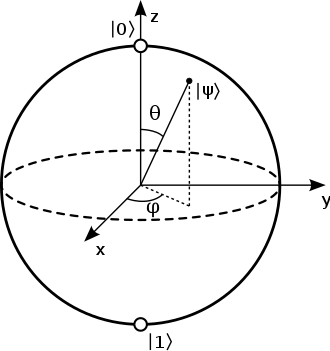
\includegraphics[scale=0.5]{bloch}
  \caption{Bloch Sphere Representation of a Qubit,}
\end{figure}

\[\alpha =  e^{i\psi}cos\dfrac{\theta}{2} \quad \& \quad \beta = e^{i(\psi + \phi)}sin\dfrac{\theta}{2} \].

\subsection{States and Entanglement}
\section{Quantum Gates}